\documentclass[tikz,11pt]{standalone}
\usepackage{lmodern}
\usepackage{amssymb}
\usepackage{pgfplots}
\pgfplotsset{compat=1.17}
\usepgfplotslibrary{external}
\usepgfplotslibrary{groupplots}
\usepgfplotslibrary{fillbetween}
\usetikzlibrary{fadings}
\begin{document}
\tikzsetnextfilename{gp-vs-lgnd}
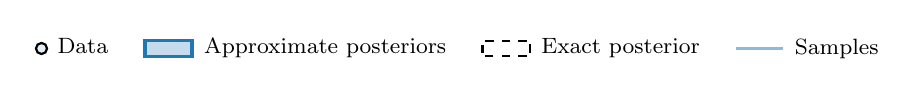
\begin{tikzpicture}
\begin{axis}[hide axis, xmin={0}, xmax={1}, ymin={0}, ymax={1}, legend columns={-1}, legend style={draw={none}, legend cell align={center}, font={\footnotesize}, column sep={0.0625cm}, /tikz/every even column/.append style={column sep=0.375cm}}]
    \addlegendimage{only marks, mark options={thick}, mark={*}, fill={rgb,1:red,0.8902;green,0.9333;blue,0.9647}}
    \addlegendentry{Data}
    \addlegendimage{fill opacity={0.25}, area legend, very thick, color={rgb,1:red,0.1216;green,0.4667;blue,0.7059}, fill={rgb,1:red,0.1216;green,0.4667;blue,0.7059}}
    \addlegendentry{Approximate posteriors}
    \addlegendimage{fill opacity={0}, area legend, thick, color={black}, dash pattern={on 0pt off 1.25pt on 3pt off 2.4375pt on 3pt off 3pt on 3pt off 3pt on 3pt off 2.4375pt on 3pt off 2.4375pt on 3pt off 3pt on 3pt off 3pt on 3pt off 3pt}}
    \addlegendentry{Exact posterior}
    \addlegendimage{opacity={0.5}, thick, color={rgb,1:red,0.1216;green,0.4667;blue,0.7059}}
    \addlegendentry{Samples}
\end{axis}
\end{tikzpicture}
\end{document}
